\chapter{Introduction}

  \section{La perception chimique}
  La perception chimique est le plus ancien système sensoriel datant de 500 millions d'années. Il fait partie des sens nécessaires à la reproduction et à l'alimentation deux des activités les plus fondamentales d'une espèce animale. Chez le poisson, la perception chimique passe par trois organes distincts sont l'olfaction, la gustation et le sens chimique commun. Contrairement aux espèces terrestres où les substances perçues par l'olfaction et la gustation diffèrent par le moyen de transport des molécules, le poisson goûte et sens par le même milieu : l'eau. De fait, c'est la solubilité des composés dans l'eau qui détermine le type de composés pouvant être transportés et perçu. La distance parcourue ainsi que la concentration (qui déterminera le seuil de perception donc le temps de résidence du composé dans l'environnement) dépendra de la diffusion du composé ainsi que le la convection du milieu. La perception chimique est très spécifique, présent à l'état de mélange dans le milieu naturel, le sens chimique étant spécifique aux structures moléculaires des composés odorants. On s'attend donc à observer des comportements d'excitation non directionnel ou des réponses orientés de remontée de gradient pour trouver des sources, par exemple pour s'orienter ou pour retrouver un lieu de ponte lors de migration. Cette navigation est une tâche complexe et ne peut s'apparenter à une simple remonté de gradient, le milieu aquatique étant en général turbulent et la perception parcellaire.
  \medbreak
  La larve de poisson-zèbre est le modèle de choix pour étudier la navigation orientée. Étant transparente à l'état larvaire, il est possible d'observer l'intégralité du cerveau avec une résolution cellulaire grâce à la microscopie à feuille de lumière pendant que l'animale effectue une tâche ce qui permet de relier les comportements à l'activité neuronale. Les organes sensoriels de la perception chimique ont été bien caractérisés chez le poisson-zèbre, il existe cependant peu d'étude comportementale sur la perception chimique et la navigation chimique. Le modèle est très utilisé dans l'étude des phénomènes d'dépendance dû au fait de la facilité de réaliser des manipulations génétique. La caractérisation d'un modèle animale pour étudier la navigation orientée par perception chimique reliant le comportement à l'activité neuronale serait un ajout puissant qui permettrait de mieux comprendre comment les poissons perçoivent et remonte à des sources de nourritures, à des conspécifiques pour la reproduction et à des sites de migration comme chez le saumon.

  \subsection{L'olfaction}
  L'organe olfactif du poisson figure~\ref{olfactory_schematic} est constitué de deux structures situées dans le museau de l'animale. Chaque structure est constituée d'une cavité appelée chambre olfactive raccordée à l'extérieur pas une narine d'entrée et une narine de sortie. L'intérieur de la chambre olfactive est tapissée de la rosette olfactive constituée de deux rangées de lamelles olfactives. L'épithélium olfactif, où sont situés les récepteurs olfactifs est placé sur ces lamelles. L'organisation exacte ainsi que la position de l'organe olfactif peut varier suivant l'espèce de poisson, avec par exemple l'ajout d'une cavité de ventilation dans le prolongement de la cavité olfactive.
  \begin{figure}[!h]
    \centering
    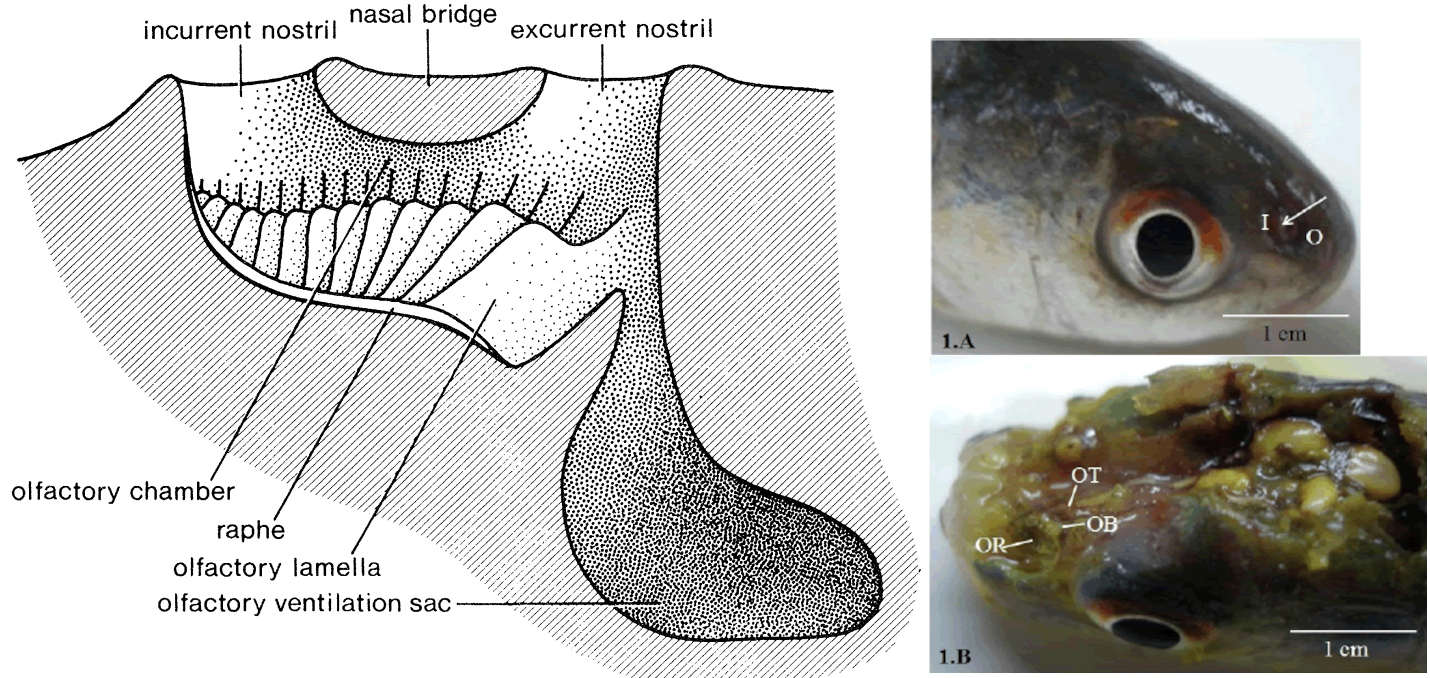
\includegraphics[width=10cm]{part_2/assets/olfactory_schematic.png}
    \caption{Le système olfactif du poisson tiré de \cite{hara2012fish}.}
    \label{olfactory_schematic}
  \end{figure}
  \medbreak
  L'épithélium olfactif à une structure en colonne stratifiée épais de $100\mu m$. Il peut être séparé en un épithélium sensoriel et un épithélium non-sensoriel. L'épithélium sensoriel est constitué de trois types de cellules : les cellules réceptrices, de supports et basales. L'épithélium non-sensoriel est constitué de cellules de Goblet et de cellules ciliées non-sensorielles.
  \medbreak
  Les cellules réceptrices sont des neurones bipolaires ciliés, microviliés \cite{ichikawa1977fine} ou pear-shaped \cite{wakisaka2017adenosine} qui expriment des récepteurs olfactifs des familles OR, V1R, V2R et TAAR. Les cellules réceptrices projettent directement dans le bulbe olfactif situé dans le cerveau, qui envoie lui-même des signaux dans le télencéphale et dans le diencéphale. Le bulbe olfactif chez les téléostes est une structure constituée de quatre couches : ONL (olfactory nerve layer), GL (glomerular layer), MCL (mitrac cell layer) et ICL (internal cell layer). L'information olfactive est transmisent par les cellules réceptrices au bulbe olfactif comme un carte topographique d'odeurs. Les connexions neuronales du bulbe olfactif ont particulièrement été étudiées chez le poisson-zèbre. Chaque cellule réceptrice exprime un seul type de récepteur olfactif. Toutes les cellules qui expriment le même récepteur projettent dans le même glomérule du bulbe olfactif. Les odeurs sont donc encodées dans une carte spatiale d'activation des glomérules. Le bulbe olfactif du poisson zèbre comprend 140 glomérules, dont 27 glomérules invariants dans leur arrangement suivant les individus \cite{braubach2012distribution}. Les axones des neurones du bulbe olfactif se terminent ensuite dans le télencéphale et le diencéphale.
  \medbreak
  Chez le poisson-zèbre \cite{hansen1993development}, l'organe olfactif se développe à partir des placodes olfactives au stade 6-10 somites (environ 15 heures après fertilisation) du développement embryonnaire. La cavité olfactive commence à apparaître au stage 28-30 somites (31 heures après fertilisation). Environ 50 heures après fertilisation, on observe l'apparition de l'épithélium olfactif et des cellules réceptrices. Quand l'embryon émerge de l'oeuf, 4 jours après fertilisation, l'organe olfactif continue son développement morphologique mais l'organisation cytologique change peu. A 40 jours après fertilisation, le pont entre la narine d'entrée et la narine de sortie se forme, séparant ainsi les courants sortant et entrant de la cavité olfactive. L'ajout de lamelles sur la rosette olfactive se poursuit tout le long de la vie du poisson zèbre.

  \subsection{La gustation}
  L'organe gustatif du poisson est constitué des papilles gustatives qui sont au contact direct des substances chimiques. Elles sont distribuées sur tout le corps du poisson et plus particulièrement dans la bouche, sur les lèvres et sur la peau. Leur distribution et leur concentration varient suivant les espèces. Elles sont innervées par 3 nerfs craniaux différents, faciale (VII), glossopharyngiale (IX) et vagale (X). Le nerf facial transmet les informations provenant des papilles gustatives extra-oral, le nerf glosopharyngial des informations provenant de l'intérieur de la cavité orale et le nerf vagal de la cavité oropharyngiale. Le système gustatif est anatomiquement divisé en deux parties distinctes, les nerfs IX et X projetant dans le lobe vagal du cerveau et le nerf IV dans le lobe facial. Les connexions à des aires plus élevées du cerveau diffèrent légèrement d'une espèce à l'autre. Il a été montré chez Ictalurus nebulosus \cite{atema1971structures} que ces deux systèmes ont des rôles distincts dans les comportements d'alimentation du poisson. Les projections du système gustatif du poisson-zèbre ont été étudié en détail \cite{yanez2017gustatory} et forme un réseau complexe qui peut être résumé graphiquement figure~\ref{gustatory_connection_schematic}.
  \begin{figure}[!h]
    \centering
    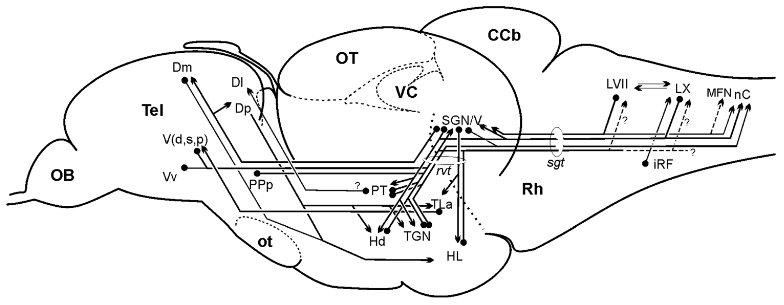
\includegraphics[width=10cm]{part_2/assets/gustatory_connection_schematic.png}
    \caption{Projection du système gustatif du poisson-zèbre tiré de \cite{yanez2017gustatory}.}
    \label{gustatory_connection_schematic}
  \end{figure}
  \medbreak
  Chez le poisson-zèbre, les papilles gustatives sont situées sur les lèvres, dans la cavité oropharyngiale, sur les barbillons et sur la face ventrale et dorsale de la tête \cite{hansen2002taste}. Les premières papilles gustatives apparaissent à 3 où 4 jours après fertilisation, elles sont situées sur les lèvres et sur les arcs branchiaux. Les papilles gustatives dans la bouche et la cavité oropharyngiale apparaissent entre 4 et 5 jours après fertilisation. Les papilles gustatives sur la tête n'apparaissent qu'à 12 jours après fertilisation et il faudra attendre l'âge juvénile (30 à 40 jours après fertilisation) pour voir l'apparition des barbillons. On remarquera que l'apparition des papilles gustatives coïncide avec l'apparition de l'alimentation autonome chez la larve.

  \subsection{Le sens chimique commun}
  Le poisson possède un troisième sens chimique nommé le sens chimique commun. Il est constitué de cellules bipolaires nommées "solitary chemosensory cells" (SCCs) présentes dans l'épiderme. Leur répartition et leur nombre varient grandement suivant les espèces.
  \medbreak
  Chez le poisson-zèbre \cite{kotrschal1997ontogeny}, les SCCs ont été décrite comme soit un ensemble de 2-7 villosités de 0.5 à 1 $\mu m$ de longueur émergeant du corps cellulaire, majoritairement présentes chez les larves, soit une seule villosité de $3\mu m$ de longueur présente en majorité chez les adultes.
  \medbreak
  Les premières SCCs apparaissent à 3 jours après fertilisation  et leur densité augmente jusqu'à 25 jours après fertilisation où leur nombre se stabilise à $1.10^6$ par $mm^2$ avec 2 à 5 fois plus de SCCs sur la tête du poisson-zèbre que sur le corps.

  \section{Réponse comportementale}
  Le poisson zèbre reste le modèle de choix pour étudier la réaction comportementale vis-à-vis de stimuli chimique. De fait, la larve de poisson zèbre est utilisé pour étudier des comportements tels que la réponse à des stimuli visuel, de chaleur, l'étude des réflexes de l'équilibre. Elle est transparente et on peut donc observer l'ensemble du cerveau grâce à un microscope à feuille de lumière et des rapporteurs calciques. On peut donc en théorie étudier facilement le lien entre réponse à un stimulu et activité neuronale.
  Pour la perception chimique, peu d'études ont été faites sur les larves de poisson zèbre, la majorité des travaux étant concentré sur le screening de drogue a visé médicale.

  \subsection{Dispositifs expérimentaux}
  L'étude comportementale de la perception chimique du poisson-zèbres, adultes où à l'état larvaire a été étudié par le biais de dispositif divers expérimentaux que nous presenterons dans la suite.
  \paragraph{Conditional place preference}
  Le conditional place preference (CPP) est un type de conditionnement Pavlovien, c’est-à-dire qu'il consiste à associer un stimulus conditionné qui a été appris à l'animale, avec un stimulus non conditionné que l'on cherche à tester. L'exemple le plus classique est d'associer le son du cloche avec le relâchement d'une odeur de nourriture. Après apprentissage l'animale répond au stimulus conditionné seul.
  Cette approche classique de psychologie a été appliquée chez le poisson-zèbres adulte pour tester la réponse à divers stimuli chimiques \cite{mathur2011conditioned}. Les expériences de ce type présentent le même dispositif expérimental et son constitué de 3 étapes. Une première étape consiste à évaluer la préférence du poisson, il est placé dans un aquarium séparé en deux ou trois parties, chaque partie présente des murs avec un motif et une couleur différente. On teste le poisson pour savoir le côté qu'il préfère, généralement on élimine les poissons ayant une trop grande préférence. La deuxième étape est celle de conditionnement, pratiqué en contraignant le poisson du côté de l'aquarium qu'il préfère le moins et en y injectant la substance à tester, cette étape peut être répétée plusieurs fois. La troisième étape de test consiste à répéter la première étape pour évaluer le changement de préférence de l'animale.
  \cite{darland2001behavioral} ont étudié la sensibilité de la cocaïne sur des poissons zèbres adultes. Ils montrent sur des poissons WT une réponse forte et robuste du CPP induite par la cocaïne avec 85\% des poissons changeant de préférence pour une concentration en cocaïne de $10mg.L^{-1}$. Les concentrations plus basses et plus hautes entraînant des réponses plus faibles. \cite{mathur2011preference} ont étudié la réponse de poissons zèbres adultes à l'éthanol dans un dispositif avec 2 chambres avec des motifs différents et une allée centrale avec un motif uniforme permettant de placer le poisson dans un environnement neutre.L'expérience dure 2 jours avec pour le premier jour la préférence de chaque poisson est calculé à partir d'un enregistrement de 5 minutes. Le deuxième jour chaque animal est conditionné avec l'éthanol dans le côté le moins préféré pendant 20 minutes et dans le côté préféré avec juste de l'eau, l'expérience étant faite en alternant l'ordre de conditionnement. Le troisième jour, la préférence de chaque animale est calculé à partir d'un enregistrement de 5 minutes. Les auteurs montrent une réponse positive au conditionnement dès une concentration de 1.5\% sans effet significatif de l'ordre du conditionnement. C'est aussi la première étude a utilisé un système automatisé de tracking pour calculer la préférence de l'animale. Des expériences similaires ont été pratiqué pour tester la réponse à divers stimuli chimiques. \cite{ninkovic2006genetic, ninkovic2006zebrafish} montrent une réponse positive au CPP pour la D-amphétamine. \cite{braida2007hallucinatory} montrent une réponse positive à la salvinorin A une substance hallucinogène, à la cocaïne et à la spiradoline. \cite{kedikian2013behavioral, } montrent une réponse positive du CPP à la nicotine et à l'éthanol.
  \medbreak
  On voit que le CPP a été beaucoup utilisé pour étudier la réponse à un stimulus chimique du poisson zèbre. L'accent est fortement mis sur des produits provoquant des pathologies d'addiction chez l'humain. Mais ce protocol présente plusieurs défauts, le premier étant qu'il repose sur un apprentissage du poisson impliquant plusieurs systèmes de perception ainsi que la mémoire. Durant la phase de conditionnement, l'apprentissage repose sur la perception visuelle de l'environnement (motif sur les murs de l'aquarium), la perception du stimulus chimique, l'association des deux stimuli provenant d'organes sensitifs différent et dans un troisième temps d'une mémorisation de ces perceptions. Deuxièmement, la mise en place du dispositif qui dure au minimum 3 jours avec une seule phase de conditionnement est un frein pour une utilisation au débit de ce système pour étudier l'effet d'un grand nombre de produits chimiques. On remarque aussi que la mise en place d'une expérience entièrement automatisée où la préférence est calculée automatiquement à partir des enregistrements des expériences a été mise en place tardivement en 2011, rendant l'analyse des expériences laborieuses avec un comptage manuel du temps passé dans chaque compartiment.
  \paragraph{Multiplates}
  Un dispositif expérimental très utilisé pour quantifier l'effet d'un composé chimique sur les larves de poissons zèbres est celui du multiplate. Une larve de poisson zèbre est placé dans chaque puit d'un multiplate et un composé chimique est introduit dans le puit. On enregistre ensuite la larve nager dans le composé chimique et on extrait les paramètres cinématiques de l'animale. L'avantage de cette technique est qu'elle nécessite peu de matériel, elle produit rapidement une grande quantité de donnée avec des multiplates allant jusqu'a 48 puits par plaque. Avec ce dispositif, de nombreux composés chimiques ont été testé pour connaitre leur toxicité.
  \paragraph{Diffusion}
  Certains auteurs ont essayé de quantifier l'effet de composé chimique en introduisant directement dans l'aquarium un composé chimique et en regardant le pourcentage de temps passé proche de la source. Notamment \cite{wakisaka2017adenosine} a montré une attraction concentration dépendante du poisson zèbre adulte à l'adénosine. L'ATP l'ADP produit par les organismes vivant sont déphosphorylés dans l'épithélium olfactif et l'adénosine résultante est perçu par une cellule sensorielle nommées pear-shaped exprimant des récepteurs spécifiques à l'adénosine. L'adénosine agit comme une substance attractive pour le poisson. \cite{krishnan2014right} montrent chez la larve de poisson zèbre une attraction concentration dépendante au GCDA. En utilisant un dispositif avec une cloison séparant deux compartiments et une zone intermédiaire où le poisson peu choisir dans quelle zone aller une attraction à la nicotine. \cite{hussain2013high} montrent avec un système en deux zones séparées et une zone intermédiaire proche de \cite{krishnan2014right} une aversion forte à la cadavérine, une odeur associée à des corps en décomposition.
  \medbreak
  Le point faible de ce type de dispositif expérimentale très facile à mettre en place est le manque de contrôle dans la concentration réelle de produit perçu par l'animale. La diffusion et la convection sont négligées dans les expériences et la concentration perçue par l'animale est mal connue et peu reproductible. \cite{hussain2013high,krishnan2014right} mitige les effets de la diffusion et convection avec une paroi séparant les deux zones, laissant toujours une incertitude dans la zone intermédiaire. De plus, ces montages exclus la réalisation d'expériences longues dû à l'homogeinisation de la concentration par diffusion. 
  \paragraph{Flux}
  Une autre classe de dispositif pour étudier la perception chimique chez le poisson zèbre est un dispositif sous flux. Divers montages expérimentaux ont été reporté dans la littérature sans qu'un standard n'émerge permettant de comparer les résultats.
  \cite{abreu2016acute, abreu2016behavioral} utilise un dispositif sous flux laminaire qui permet de séparer un aquarium en 2 compartiments distincts sans mur physique testé dans \cite{readman2013fish}. L'animale peut alors choisir entre les deux compartiments sans contraintes. Plusieurs substances psychoactives ont été testé sur des poissons zèbre adultes, le temps passé dans le produit, le nombre de croisements ainsi que les paramètres cinématiques de l'animale sont enregistrés. Ils montrent une attraction par le diazepam, fluoxetine, risperidome et buspirone. Une aversion pour les pH acide et pour deux extraits d'odeurs de nourriture. Un comportement neutre pour l'éthanol. Aucun changement dans la paramètres cinématique de nage  sauf pour les deux extraits d'odeurs de nourriture. Toujours avec le même dispositif expérimental, les auteurs testent l'attraction ou la répulsion face à une eau conditionnée. Dans un premier temps, des poissons sont placés dans un aquarium et soumis soit à un stress chimique (diminution du pH), soit à un stress physique (chasser par un filet), soit à une image de prédateur où enfin à une privation de nourriture plus où moins importante. Dans un deuxième temps, des poissons sont testés dans le dispositif à flux laminaire pour regarder la préférence à cette eau conditionnée. Les auteurs trouvent une aversion significative pour l'eau conditionnée par un stress chimique et physique. Aucune différence significative est trouvé pour le conditionnement par l'image d'un  prédateur. Ils montrent une aversion pour l'eau conditionnée avec des poissons privés de nourriture pendant 48 heures et aucune différence pour des poissons suivant un nourrissage normal où un jeun chronique.
  \medbreak
  \cite{kermen2020stimulus} utilisent un dispositif à flux qui au lieu de séparer l'aquarium en deux parties distinctes permet de rapidement changer la concentration en produit dans l'intégralité de l'aquarium. En enregistrant les paramètres cinématiques de l'animale, ils peuvent ensuite conclure sur l'impact du composé chimique. Les résultats ne sont plus cette fois-ci exprimés en terme d'attraction répulsion mais peuvent être comparé à ceux du multiplate, l'intérêt étant de pouvoir faire l'expérience avec des animaux adultes qui nécessites un grand volume d'eau en trois dimensions pour évoluer de manière réaliste. Avec ce dispositif, les auteurs montrent que les poissons modulent leur trajectoire en influant sur 7 paramètres indépendants que sont la vitesse, le nombre de burst, le nombre de virages, le déplacement horizontal et vertical, le temps passé figé ainsi que la position verticale. À partir de ces valeurs, ils peuvent classer les odeurs en regroupant celle entraînant la même réponse comportementale. Les odeurs de nourritures entraîne une augmentation significative de la vitesse et du nombre de burst, les odeurs sociales (provenant d'autres poissons) entraîne une réponse similaire à celle des odeurs de nourriture, les odeurs d'alertes entraîne une descente vers le fond de l'aquarium et une augmentation du temps passé figé, et les odeurs de décomposition entraîne plus de virage.
  Le point essentiel relevé par cette étude est la variabilité inter et intra expérience. Les auteurs montrent que moins d'un tier des odeurs utilisées dans l'étude produisent des résultats reproductible entre essai d'un même individu. Certaines odeurs comme la cadavérine, le sang, la peau et les odeurs de nourriture entraîne des réponses consistantes pour un même individu. Le plupart des odeurs produisent des résultats peu reproductibles pour différents poissons (corrélation inférieure à 0.5). 
  Ce type de dispositif expérimentale permet une meilleure gestion de la concentration perçue par l'animale qui est parfaitement contrôlé après un régime transitoire de mise en place. Elle permet aussi la réalisation d'expériences longues, le flux permettant de stopper la diffusion et la convection du composé chimique.
  \medbreak
  On voit donc à travers cet aperçu de la littérature scientifique que l'étude de la perception chimique et de la réponse comportementale au stimulus chimique n'est pas standardisé. Aucun montage expérimental n'est standardisé et ne permet une comparaison directe entre les études effectuées dans divers laboratoires indépendants. C'est dans ce contexte que nous avons mis au point Dual, un montage expérimental facile à construire soit-même, documenté et permettant d'étudier de manière standardisée et comparable la réponse comportementale chez la larve et le poisson-zèbre juvénile.


\chapter{Dispositif expérimental}

  \section{Dual}
  \subsection{Introduction}
  La reproductibilité des études comportementales est un problème ouvert en neuroscience. La conception et la réalisation de montages expérimentaux permettant un grand débit d'expériences en d'éviter tout biais est essentielle à la caractérisation d'un comportement. L'absence de standard en matière d'étude de la réponse comportementale à des stimuli chimiques ne permet pas à ce jour de comparer facilement les résultats obtenus au travers des diverses études menées jusqu'à présent. C'est dans ce contexte que nous présentons Dual, un montage expérimental à haut débit d'expérience facile à réaliser et à mettre en place.
  \medbreak
  On verra dans un premier temps la philosophie du dispositif, dans quel but il a été conçu et pour quelle utilisation. Dans un second temps les étapes de construction et enfin on verra son utilisation et son coût en temps pour réaliser une campagne d'expérience.
  \subsection{Philosophie}
  Dual est un système du même type que \cite{readman2013fish} qui consiste à créer grâce à un flux laminaire deux compartiments virtuels dans l'aquarium. Comme on l'a vu précédemment, ce système permet une connaissance rigoureuse de la concentration du composé chimique auquel est soumis l'animale. Il permet aussi d'éviter la convection due au mouvement d'eaux engendré par la nage du poisson, toutes les perturbations étant entraînées par le flux. On a donc deux compartiments virtuels bien défini par une interface qui se "répare" d'elle-même dans un temps caractéristique donné par la vitesse de l'écoulement laminaire. 
  \medbreak
  Pour se faire, Dual utilise un système de quatre seringues (2 seringues infectantes et 2 seringues aspirantes) qui permet de créer un flux laminaire constant dans l'aquarium où évolue le poisson. Le rôle des seringues peut être inversés grâce à un système de valves pour pouvoir les remplir et choisir le produit qu'elles contiennent. On peut alors construire une expérience en réalisant plusieurs cycles de remplissage-injection. Par exemple en aspirant en premier de l'eau dans les deux seringues ce qui constituera en injection un flux laminaire d'eau homogène (contrôle) et dans un second temps un produit dans une seringue et de l'eau dans l'autre ce qui en injection permettra de créer un flux laminaire de produit et un flux laminaire d'eau créant deux compartiments virtuels dans l'aquarium. 
  \medbreak
  Dual est inspiré du mouvement Do It Yourself qui permet de construire des choses sans l'aide d'expert du domaine. C'est dans ce sens que tous les composants, plans et autres fichiers CAD nécessaires à la création et au montage de Dual sont disponibles en annexe. Dual peut être construite à moindre coût sans connaissance préalable en mécanique ou en électronique. Les machines nécessaires à la réalisation des pièces peuvent être trouvé dans un FabLab et à moindre coût.
  \subsection{Construction}
  \paragraph{Overview}
  Dual est constitué de quatre parties distinctes : une partie mécanique, une partie hydraulique, une partie électronique et enfin un logiciel informatique permettant de contrôler tout le dispositif.
  \paragraph{Système mécanique}
  La partie mécanique de Dual comprend un pousse seringue motorisé, un support de caméra et un aquarium isolé de l'environnement extérieur. Le pousse-seringue motorisé permet d'accommoder quatre seringues figure~\ref{} qui marche deux à deux en opposition de phase. Quand les seringues supérieures injectent, les seringues inférieures se remplissent et inversement. Cela va permettre de créer le flux laminaire nécessaire à la création des deux compartiments virtuels. Tous les plans et fichiers nécessaires à la réalisation des différents éléments est disponible en annexe.
  \medbreak
  L'aquarium figure~\ref{} est constitué d'une puce millifluidique en XXXX réalisée à la découpe laser et coller grâce à de l'acide acétique. Le XXXX est un matériau plastique transparent ce qui permet de conserver une bonne qualité d'image quand on filme en transmission. Elle est constituée en son centre d'une zone délimitée par deux grilles en plastique réalisées en impression 3D où le poisson pourra évoluer. La puce comprend deux entrées et deux sorties qui seront connectées par le système hydraulique aux seringues. Cela permet de créer deux flux laminaires à volume constant dans l'aquarium. Le tronçon reliant les entrées et les sorties à la zone où le poisson est confinée présente un profil évasé pour éviter toutes perturbations et un raccordement optimal entre les deux flux laminaires. Enfin, une plaque en plastique est placée au-dessus du système et permet d'éviter que le poisson ne s'échappe et les déformations optiques lors de l'enregistrement.
  \medbreak
  La puce millifluidique est placée dans une boîte réalisée avec une structure en MakerBeam et des panneaux en MDF découpé à la découpe laser. Cette boîte permet d'isoler l'expérience du milieu environnant et de placer l'animale dans un éclairage contrôlé (ou bien obscurité complète). Cette boîte contient figure~\ref{} de bas en haut : deux LED permettant d'éclairer en lumière visible et en infrarouge (nécessaire pour l'enregistrement), un diffuseur permettant un éclairage homogène, la puce microfluidique et sur la face supérieure une fenêtre amovible constituée d'un filtre laissant uniquement passer la lumière IR, cela permet de bloquer toutes lumières extérieures tout en pouvant enregistrer les images de l'expérience en lumière IR.
  \medbreak
  Un support de caméra est placé au-dessus de la boîte et une caméra Chameleon3 FLIR Systems permet d'enregistrer les expériences en lumière IR.
  \medbreak
  Tous ces éléments sont fixés solidement et à niveau à la table pour éviter toutes vibrations ou biais qui pourraient perturber l'animale pendant l'expérience. La facilité de réalisation de la puce microfluidique en moins de 12 h permet de la remplacer facilement en cas de détérioration ou de contamination.
  \paragraph{Système hydraulique}
  Le système hydraulique permet de relier les seringues à la puce microfluidique avec un système de valves permettant de choisir quelle seringue injectera dans quelle entrée de la puce microfluidique, et depuis quel récipient se remplira la seringue, un schéma du circuit est disponible figure~\ref{}. Ce système permet de créer des expériences construites en mettant bout à bout des cycles de remplissage et d'injection. Les valves sont contrôlées électroniquement ce qui permet d'automatiser complétement le système.
  \paragraph{Système électronique}
  Le système électronique permet de faire l'interface entre les éléments à contrôler que sont les valves, les LED et le moteur du pousse-seringue et le logiciel informatique. Le circuit imprimé a été créé sur-mesure~\ref{}. Il accueille un Arduino Nano servant de microcontrôleur, Six relais permettant le contrôle des valves à partir des signaux logiques de l'Arduino. Un contrôleur de moteur pas à pas EasyDriver permettant de contrôler la vitesse du moteur depuis une sortie logique de l'Arduino. Un système de potentiomètre permet de contrôler l'intensité des LED d'éclairage. Tout le système électronique ainsi que le moteur du pousse-seringue est alimenté par une alimentation ATX d'ordinateur 550W connectée au circuit imprimé par un montage inspiré du Benchtop Power Board de Sparkfun.
  \paragraph{Système informatique}
  Un logiciel a été développé spécialement pour contrôler le dispositif. L'interface graphique a été créée à l'aide de Qt et la caméra est interfacé au logiciel grâce au SDK de FLIR Systems. Le logiciel permet de contrôler manuellement chaque élément du système comme les valves, la caméra et le moteur du pousse-seringue. Il permet de contrôler l'éclairage ainsi que d'enregistrer les images provenant de la caméra. Il est possible (et conseillé) de créer des templates d'expériences, un simple fichier texte, contenant les instructions nécessaires à l'automatisation des cycles d'injection et d'aspiration. Le logiciel permet de contrôler depuis la même interface quatre Duals.
  \subsection{Utilisation}
  Pour nos besoins, nous avons construit quatre Duals que nous avons fait tourner en parallèle. La construction complète du montage nécessite une découpe laser, une imprimante 3D, du matériel électronique (fer à souder, etc.) et du matériel d'atelier (tournevis, vis, perceuse, etc.) et les matériaux et plan (disponible en annexe ~\ref{}. Deux semaines ont été nécessaires à la construction du dispositif à partir des plans. La construction ne demande pas de connaissance spécifique et la construction par exemple dans un FabLab permettra de trouver le matériel et l'aide nécessaire en cas de difficultés à réaliser le projet.
  \medbreak
  L'utilisation du Dual est extrêmement simple en pratique. Une fois le template d'expériences créé, la seule tâche manuelle est de placer le poisson dans la puce microfluidique, de refermer le dispositif et de faire jouer le template d'expérience. Il est nécessaire de contrôler que les récipients d'aspiration (eau où produit) sont remplis. Il est alors possible d'enchaîner les expériences avec peu de temps mort et une intervention manuelle minimale.
  \medbreak
  Un problème récurrent que nous avons rencontré est l'encrassage du circuit hydraulique. Le colorant utilisé pour visualiser l'écoulement~\ref{} fini par boucher les valves. Une solution trouvée est de régulièrement passer les valves dans un bain ultrasonique pour les déboucher et de changer de temps en temps les tuyaux qui raccordent les valves, les seringues et la puce microfluidique. Le fait d'effectuer un protocole de rinçage qui peut être lancé automatiquement à la fin de la journée nous a aussi permis de réduire ce problème. 

  \section{The Tropical River}
  \subsection{Description}
  La perception chimique dans un environnement aquatique turbulent comme lequel sont soumis les poissons nécessite un dispositif expérimental permettant de créer de manière contrôlé des écoulements et de délivrer des stimuli chimique. Pour se faire, nous avons créé un dispositif expérimental permettant de délivrer un écoulement laminaire à température contrôlée, permettant d'imager les poissons aussi bien en lumière visible qu'en lumière infrarouge pour les placer dans le noir total. Une buse d'injection permet de créer des panaches turbulent ou laminaire à l'intérieur de cet écoulement.
  \paragraph{Dispositif mécanique}
  La partie mécanique du dispositif est constitué d'un canal assemblé à partir de plaque de PVC transparent. Une plaque lumineuse est placé sous le canal permettant un éclairage en lumière visible par le dessous pour éviter toutes réflexions sur la surface de l'eau. Le canal peut être éclairé par le dessus par un ensemble de LED infrarouge. Une caméra est placée au-dessus du canal et permet d'enregistrer les expériences. Un miroir est placé à 45 degrés sur le côté du canal ce qui permet de récupérer les positions verticales des poissons sur la même image que leurs positions horizontales. L'ensemble du canal est placé dans une boîte pour l'isoler de la lumière et de toutes perturbations liées à l'environnement immédiat de l'expérience.
  \paragraph{Dispositif hydrodynamique}
  Le canal est alimenté en eau depuis un robinet connecté au réseau d'eau du bâtiment. Avant d'arriver dans le canal, elle est filtrée par un filtre au charbon actif, chauffé grâce à un système de bain marie puis injecté par une extrémité du canal. Un réseau de paille est placé dans le canal permettant ainsi de régulariser l'écoulement turbulent en écoulement laminaire. Le débit peut être ajusté grâce à une valve solénoïde. L'autre extrémité du canal est laissé libre et l'eau sortante est redirigé vers le réseau d'eau usé du bâtiment, les produits testés ne nécessitant pas de traitement particulier. Il est possible de diluer un produit en amont du canal grâce à une buse d'injection située directement à la sortie de l'alimentation en eau, un agitateur magnétique est placé directement dans le canal pour faciliter la dilution. Une autre buse d'injection peut être placé dans le canal pour créer un panache dans l'écoulement, il est alimenté depuis un réservoir placé en hauteur et le débit peut être ajusté par gravité.
  \paragraph{Dispositif de contrôle}
  Tous les composants du système sont contrôlés depuis un logiciel maison.
  \subparagraph{Température}
  Un capteur de température est placé dans l'écoulement et envoie la température instantanée au logiciel de contrôle. Le logiciel va alors sélectionner la température du bain marie en amont de l'injection dans le canal grâce à un système de rétro action par PID. Cela permet de garder une température constante de le canal malgré des variations de température dans le système d'eau du bâtiment.
  \subparagraph{Injection}
  L'injection de différent produit peut être sélectionné de manière automatisé grâce à un système de valves contrôlé par le logiciel. Cela permet de mettre en place facilement des protocoles d'injection. La vitesse de l'écoulement laminaire dans le canal est aussi configurable dans le logiciel et est modulé grâce au contrôleur de débit à l'entrée du dispositif.
  \subparagraph{Caméra}
  Le réglage et l'acquisition des images par la caméra est fait directement dans le logiciel de contrôle, ce qui permet d'inclure dans les fichiers des données tel que le temps relatif à l'expérience, la température instantanée et d'autres variables.
  \paragraph{Logiciel}
  Le logiciel de contrôle permet de récupérer et de contrôler toutes les variables de l'expérience. Il permet de sélectionner la vitesse, la température de l'écoulement et les paramètres de capture de la caméra. Une fonction clef du logiciel est de pouvoir construire des protocoles d'expérience. Il s'agit de simple fichier texte précisant la valeur souhaitée des variables a un temps donné. Le logiciel accepte nativement d'autres capteurs Arduino répondant à un standard prédéfini permettant de facilement rajouter un ou des capteurs sans avoir à modifier le logiciel.
  \subsection{Utilisation et limitation}
  On voit que ce dispositif expérimental est très versatile. La capacité à moduler séparément ou simultanément la vitesse, la température de l'écoulement laminaire, ainsi que l'injection de produits dans l'écoulement de manière automatisée et quantifiée tout en filmant les poissons à la lumière ou dans le noir permet d'étudier une grande variété de comportement de rhéotaxie à la chimiotaxie en passant par la thermotaxie.
  La hauteur d'eau dans le canal peut être modulé par l'ajout d'une digue en sortie ce qui permet de faire évoluer dans le canal des larves ainsi que des poissons zèbres adultes sans difficulté.
  \paragraph{Limitations}
  L'insertion dans l'écoulement de produit chimique ne nous permet pas de réutiliser l'eau après passage dans le canal, c'est pour cela que l'apport d'eau est effectué via le réseau d'eau du bâtiment. Bien que filtré, la qualité de l'eau dépend de celle du réseau ce qui ne pose pas en principe de problème pour les poissons juvéniles et adultes qui sont élevés dans l'eau du robinet filtrée dès 2 semaines. Cela peut en revanche posé plus de problème pour les larves qui sont plus fragiles et nécessite une eau calibrée particulière (E3).
  Bien qu'en principe la durée de l'expérience n'a comme limite que l'espace de stockage disponible à l'enregistrement des images, on remarque au bout de quelque heure l'apparition de bulles de le canal qui viennent perturber les poissons, l'ajout du filtre au charbon actif permet une diminution de ce phénomène mais il reste présent.


\chapter{Résultats}
